% Diving log book page
% Author: Slava <rayslava@gmail.com> Barinov
% License: Creative Commons CC BY 4.0
% Based on original dive log page from http://texblog.org/2015/07/22/diy-scuba-diving-log-book/
%
% Template: two-sided A5 page for printing on A4 paper
% Printing:
% - A4
% - Short side binding
% - No scale, print original size
% - Recommended paper: 120 - 140 g/m2

\documentclass[a5paper,14pt]{extarticle}
\usepackage{fouriernc,parskip}
\usepackage{forloop}
\usepackage{tikz}
\usepackage[margin=3mm,left=-1.7cm, right=1.8cm,portrait]{geometry}
\usepackage{pgfpages}
\usepackage{textcomp}
\usepackage{xcolor}
\usepackage{utfsym}
\usepackage[pages=some]{background}

% Set up grid for perfect measurements
% \usepackage[grid, gridunit=mm, gridcolor=blue!10, subgridcolor=blue!15]{eso-pic}

\pgfpagesuselayout{2 on 1}[a4paper,landscape,border shrink=5mm]

\usepackage[most]{tcolorbox}
\usepackage{afterpage}
\usetikzlibrary{positioning}
\usetikzlibrary{calc}

\tcbset{
  frame code={}
  center title,
  left=0pt,
  right=0pt,
  top=5pt,
  bottom=0pt,
  colback=gray!15,
  colframe=white,
  width=\dimexpr\textwidth\relax,
  enlarge left by=0mm,
  boxsep=5pt,
  arc=5pt,outer arc=5pt,
}

\linespread{2}

% Background is CC BY from https://commons.wikimedia.org/wiki/File:World_Map_Grayscale.png
\backgroundsetup{
  scale=.6,
  color=black,
  opacity=.2,
  angle=270,
  hshift=-6em,
  contents={%
    \includegraphics[width=2\paperwidth,height=.85\paperheight]{World_Map_Grayscale.png}
  }%
}

% Shaded color for captions
\definecolor{grayedcaption}{gray}{.5}
\definecolor{boundbox}{gray}{.4}
\definecolor{dashbox}{gray}{.6}

\begin{document}
\newgeometry{margin=3mm,left=.8cm}
\newcounter{counter}
\forloop{counter}{0}{\value{counter} < 2}{
  \thispagestyle{empty}
  \begin{tikzpicture}[overlay, thin]
    \draw [draw=dashbox,dashed]  ($(current page.south west) + (-.8cm,-0.1cm)$) circle (2mm) node {};
    \draw [draw=dashbox,dashed]  ($(current page.south west) + (-.8cm,-7.6cm)$) circle (2mm) node {};
    \draw [draw=dashbox,dashed]  ($(current page.south west) + (-.8cm,-15.1cm)$) circle (2mm) node {};
  \end{tikzpicture}
  \BgThispage
  \noindent
  \vspace{-1em}
  \begin{minipage}{0.6\linewidth}
    \noindent
    \centering
    Dive No. \hrulefill~Date \hrulefill\\
    Location \hrulefill\\
    Dive site \hrulefill
  \end{minipage}
  \qquad
  \begin{minipage}{0.4\linewidth}
    \hspace{-1.7em}
    \fbox{\parbox[c][9.7em][c]{9.7em}{\hspace{9.7em}}}\\
    {\scriptsize \textcolor{grayedcaption}{Stamp}}
  \end{minipage}
  \vspace{-2em}
  \noindent
  \begin{minipage}{0.58\linewidth}
    \vspace{1.2em}
    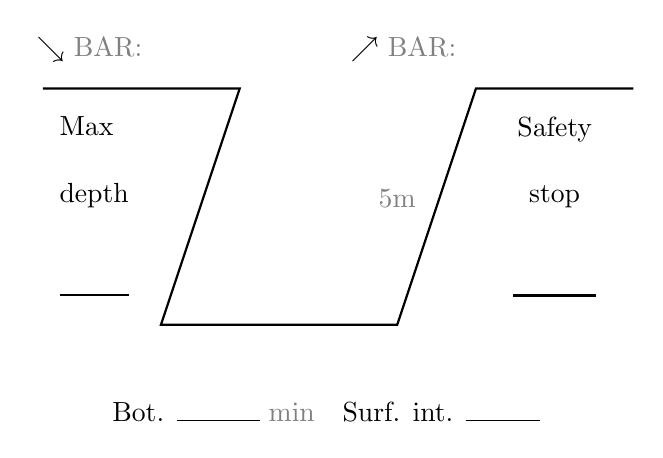
\begin{tikzpicture}
      \draw[thick] (0,0) -- (2.5,0) -- (1.5,-3) -- (4.5,-3) -- (5.5,0) -- (7.5,0);
      \node [text width=.5em, align=center] (time) at (.3,-1.5) {\baselineskip=24pt Max\\depth\vspace{1em}\\\rule{2.5em}{0.8pt}\par};
      \node [text width=1em, align=right] (entry) at (.1,.5) {\baselineskip=24pt $\searrow$~\textcolor{grayedcaption}{BAR:}\par};
      \node [text width=.5em, align=center] (entry) at (4,.5) {\baselineskip=24pt $\nearrow$~\textcolor{grayedcaption}{BAR:}\par};
      \node [align=center] (depth) at (3.6,-4.1) {Bot. \rule{3em}{0.5pt}\ \textcolor{grayedcaption}{min}\hspace{1em}Surf. int. \rule{2.7em}{0.5pt}};
      \node [text width=3em, align=center] (stop) at (6.5,-1.5) {\baselineskip=24pt Safety\\stop\vspace{1em}\\\rule{3em}{0.8pt}\par};
      \node [align=center] (stop3) at (4.5,-1.4) {\textcolor{grayedcaption}{5m}};
    \end{tikzpicture}
  \end{minipage}
  \quad
  \begin{minipage}{0.38\linewidth}
    \vspace{1em}
    \noindent
    \centering
    $\square$ Long $\square$ Short $\square$ Dry \\
    \phantom{}\hrulefill\ mm~EAN\hrulefill\\
    Weights \hrulefill\\
    {\Large \usym{1F321}}\textdegree C \hrulefill Vis: \hrulefill\\
    TABT \hrulefill~\textbf{:}~\hrulefill\\
  \end{minipage}

  \vspace{4em}
  \noindent
  \phantom{}\hrulefill\\
  \phantom{}\hrulefill\\
  \phantom{}\hrulefill\\
  \phantom{}\hrulefill\\
  \phantom{}\hrulefill\\\vspace{-3em}
  \begin{tcolorbox}
    {\vspace{-.5em}\footnotesize \textcolor{grayedcaption}{Verification}}\vspace{-1em}\\
    Name \hrulefill\ Cert~No.~\hrulefill\\
    Sign \hrulefill~$\square$ Instructor $\square$ Dive master $\square$ Buddy
  \end{tcolorbox}
  \clearpage
}

\restoregeometry
\forloop{counter}{0}{\value{counter} < 2}{
  \thispagestyle{empty}
  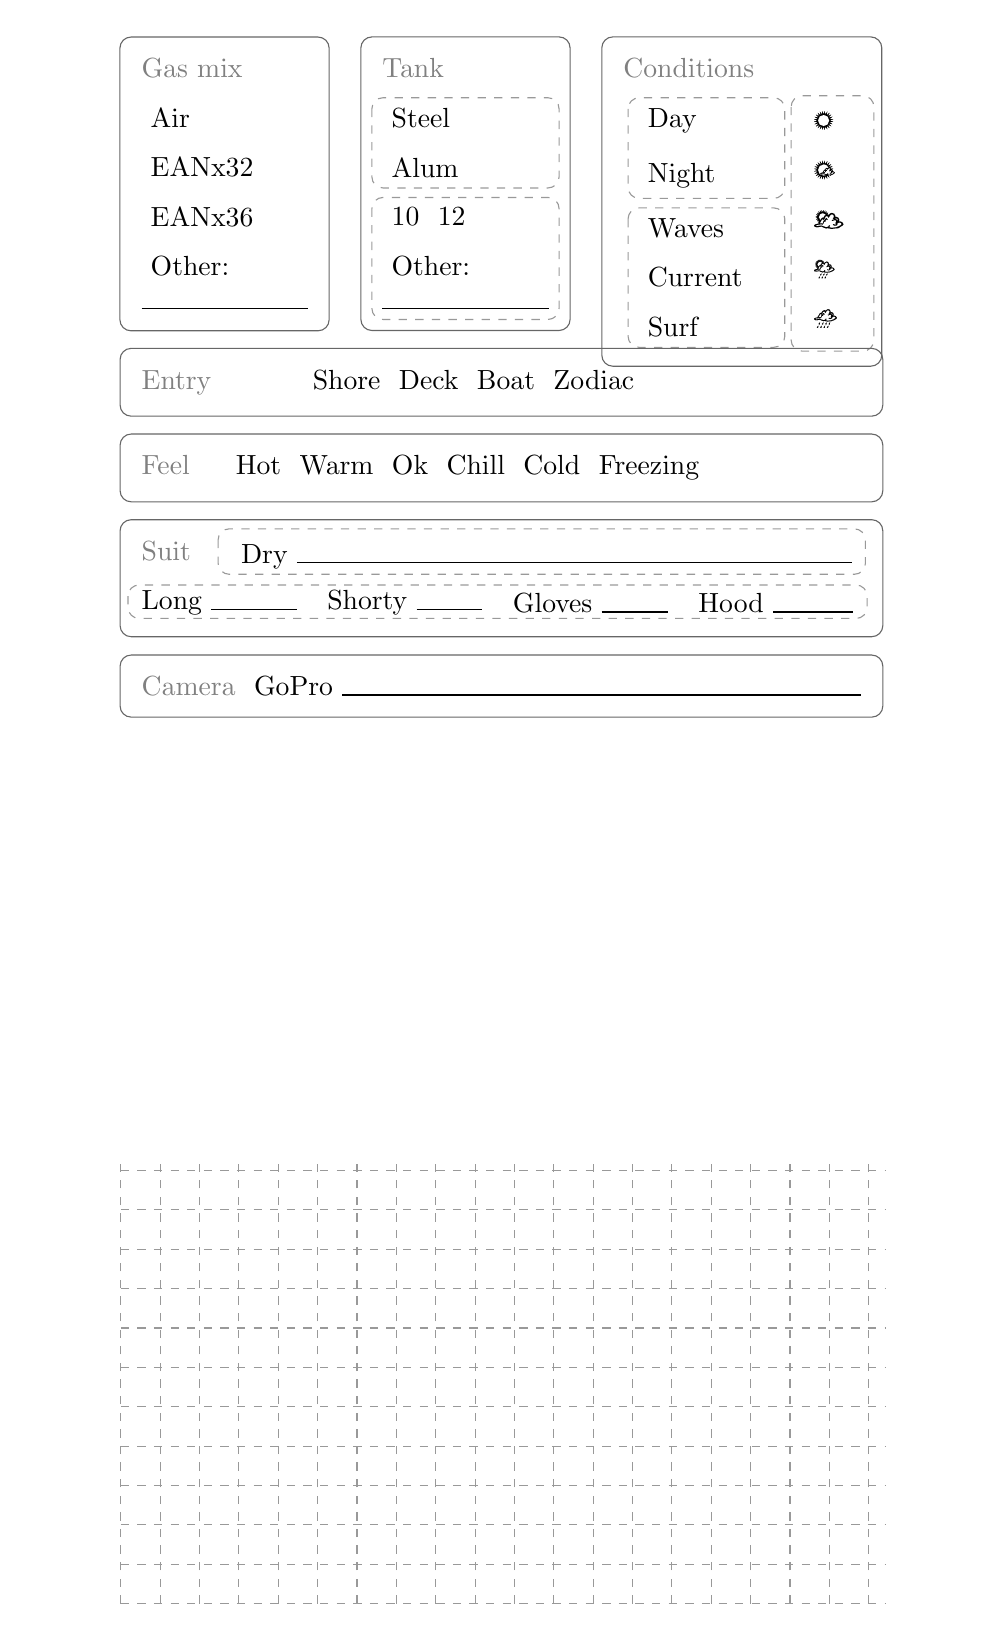
\begin{tikzpicture}[node distance=0.4em,text width=6em]
    % We need layers to draw the block diagram
    \pgfdeclarelayer{background}
    \pgfdeclarelayer{foreground}
    \pgfsetlayers{background,main,foreground}

    % Gas mix part
    \node [align=left] (mix) {\textcolor{grayedcaption}{Gas mix}};
    \node [align=left, below = of mix] (air) {$\square$~Air};
    \node [align=left, below = of air] (ean32) {$\square$~EANx32};
    \node [align=left, below = of ean32] (ean36) {$\square$~EANx36};
    \node [align=left, below = of ean36] (custmix) {$\square$~Other:\\\phantom{}\hrulefill};

    \begin{pgfonlayer}{background}
      % Compute a few helper coordinates
      \pgfmathsetmacro{\sp}{0.15}
      \path (mix.west |- mix.north)+(-\sp,\sp) node (a) {};
      \path (custmix.south -| custmix.east)+(+\sp,-\sp) node (b) {};
      \path[rounded corners, draw=boundbox, solid]
      (a) rectangle (b);
    \end{pgfonlayer}

    % Tank part
    \node [align=left, right = 2em of mix] (tank) {\textcolor{grayedcaption}{Tank}};
    \node [align=left, below = of tank] (steel) {$\square$~Steel};
    \node [align=left, below = of steel] (al) {$\square$~Alum};
    \node [align=left, below = of al] (vol) {$\square$~10~$\square$~12};
    \node [align=left, below = of vol] (othtank) {$\square$~Other:\\\phantom{}\hrulefill};

    \begin{pgfonlayer}{background}
      % Compute a few helper coordinates
      \pgfmathsetmacro{\sp}{0.15}
      \path (tank.west |- tank.north)+(-\sp,\sp) node (a) {};
      \path (othtank.south -| othtank.east)+(+\sp,-\sp) node (b) {};
      \path[rounded corners, draw=boundbox, solid]
      (a) rectangle (b);

      \pgfmathsetmacro{\sp}{0.01}
      \path (steel.west |- steel.north)+(-\sp,\sp) node (a) {};
      \path (al.south -| al.east)+(+\sp,-\sp) node (b) {};
      \path[rounded corners, draw=dashbox, dashed]
      (a) rectangle (b);

      \pgfmathsetmacro{\sp}{0.01}
      \path (vol.west |- vol.north)+(-\sp,\sp) node (a) {};
      \path (othtank.south -| othtank.east)+(+\sp,-\sp) node (b) {};
      \path[rounded corners, draw=dashbox, dashed]
      (a) rectangle (b);
    \end{pgfonlayer}

    % Conditions part
    \node [align=left, right = 2em of tank] (conditions) {\textcolor{grayedcaption}{Conditions}};
    \node [align=left, text width = 4.9em, below = of conditions] (day) {$\square$~Day};
    \node [align=left, text width = 4.9em, below = of day] (night) {$\square$~Night};

    \node [align=left, text width = 2em, right = of day] (sun) {$\square$~\usym{1F323}};
    \node [align=left, text width = 2em, below = of sun] (lightcloud) {$\square$~\usym{1F324}};
    \node [align=left, text width = 2em, below = of lightcloud] (cloud) {$\square$~\usym{1F325}};
    \node [align=left, text width = 2em, below = of cloud] (rain) {$\square$~\usym{1F326}};
    \node [align=left, text width = 2em, below = of rain] (hardrain) {$\square$~\usym{1F327}};

    \node [align=left, text width = 4.9em, below = of night] (wave) {$\square$~Waves};
    \node [align=left, text width = 4.9em, below = of wave] (current) {$\square$~Current};
    \node [align=left, text width = 4.9em, below = of current] (surf) {$\square$~Surf};

    \begin{pgfonlayer}{background}
      % Compute a few helper coordinates
      \pgfmathsetmacro{\sp}{0.15}
      \path (conditions.west |- conditions.north)+(-\sp,\sp) node (a) {};
      \path (surf.south -| rain.east)+(+\sp,-\sp-.1) node (b) {};
      \path[rounded corners, draw=boundbox, solid]
      (a) rectangle (b);

      \pgfmathsetmacro{\sp}{0.01}
      \path (day.west |- day.north)+(-\sp,\sp) node (a) {};
      \path (night.south -| night.east)+(+\sp,-\sp) node (b) {};
      \path[rounded corners, draw=dashbox, dashed]
      (a) rectangle (b);

      \pgfmathsetmacro{\sp}{0.05}
      \path (sun.west |- sun.north)+(-\sp,\sp+.02) node (a) {};
      \path (hardrain.south -| hardrain.east)+(+\sp,-\sp-.12) node (b) {};
      \path[rounded corners, draw=dashbox, dashed]
      (a) rectangle (b);

      \pgfmathsetmacro{\sp}{0.01}
      \path (wave.west |- wave.north)+(-\sp,\sp) node (a) {};
      \path (surf.south -| surf.east)+(+\sp,-\sp) node (b) {};
      \path[rounded corners, draw=dashbox, dashed]
      (a) rectangle (b);
    \end{pgfonlayer}

    % Water entry part
    \node [align=left, below = 1.5em of othtank,xshift=1.3em, text width=26em] (entry) {\textcolor{grayedcaption}{Entry\hspace{3em}} $\square$~Shore~$\square$~Deck~$\square$~Boat~$\square$~Zodiac};
    \begin{pgfonlayer}{background}
      % Compute a few helper coordinates
      \pgfmathsetmacro{\sp}{0.15}
      \path (entry.west |- entry.north)+(-\sp,\sp) node (a) {};
      \path (entry.south -| entry.east)+(+\sp,-\sp) node (b) {};
      \path[rounded corners, draw=boundbox, solid]
      (a) rectangle (b);
    \end{pgfonlayer}

    % Feeling part
    \node [align=left, below = 1.5em of entry, text width=26em] (feeling) {\textcolor{grayedcaption}{Feel\hspace{1em}} $\square$~Hot~$\square$~Warm~$\square$~Ok~$\square$~Chill~$\square$~Cold~$\square$~Freezing};
    \begin{pgfonlayer}{background}
      % Compute a few helper coordinates
      \pgfmathsetmacro{\sp}{0.15}
      \path (feeling.west |- feeling.north)+(-\sp,\sp) node (a) {};
      \path (feeling.south -| feeling.east)+(+\sp,-\sp) node (b) {};
      \path[rounded corners, draw=boundbox, solid]
      (a) rectangle (b);
    \end{pgfonlayer}

    % Suit part
    \node [align=left, below = 1.5em of feeling, text width=26em] (suit)
    {\textcolor{grayedcaption}{Suit}};

    \node [align=left, text width=5.6em, xshift = -10.2em, below = of suit] (long) {Long~\hrulefill};
    \node [align=left, text width=5.6em, right = of long] (shorty) {Shorty~\hrulefill};
    \node [align=left, text width=5.6em, right = of shorty] (gloves) {Gloves~\hrulefill};
    \node [align=left, text width=5.6em, right = of gloves] (hood) {Hood~\hrulefill};

    \node [align=left, text width = 22.4em, xshift = -23.85em, yshift=-.2em, right = of suit] (dry) {$\square$~Dry~\hrulefill};

    \begin{pgfonlayer}{background}
      % Compute a few helper coordinates
      \pgfmathsetmacro{\sp}{0.15}
      \path (suit.west |- suit.north)+(-\sp,\sp) node (a) {};
      \path (long.south -| feeling.east)+(+\sp,-\sp) node (b) {};
      \path[rounded corners, draw=boundbox, solid]
      (a) rectangle (b);


      \pgfmathsetmacro{\sp}{0.05}
      \path (dry.west |- dry.north)+(-\sp,\sp+.02) node (a) {};
      \path (dry.south -| dry.east)+(+\sp,-\sp+.10) node (b) {};
      \path[rounded corners, draw=dashbox, dashed]
      (a) rectangle (b);

      \pgfmathsetmacro{\sp}{0.05}
      \path (long.west |- long.north)+(-\sp,\sp-.1) node (a) {};
      \path (hood.south -| hood.east)+(+\sp,-\sp+.1) node (b) {};
      \path[rounded corners, draw=dashbox, dashed]
      (a) rectangle (b);
    \end{pgfonlayer}

    % Photo part
    \node [align=left, below = 3.5em of suit, text width=26em] (photo)
    {\textcolor{grayedcaption}{Camera~}$\square$~GoPro~\hrulefill};
    \begin{pgfonlayer}{background}
      % Compute a few helper coordinates
      \pgfmathsetmacro{\sp}{0.15}
      \path (photo.west |- photo.north)+(-\sp,\sp) node (a) {};
      \path (photo.south -| photo.east)+(+\sp,-\sp) node (b) {};
      \path[rounded corners, draw=boundbox, solid]
      (a) rectangle (b);
    \end{pgfonlayer}

    \draw[step=5mm,dashbox,dashed,thin,xshift=-3.75em,yshift=-19.5cm] (0, 0) grid (27.63em, 15.95em);
  \end{tikzpicture}

  \backgroundsetup{
    scale=.6,
    color=black,
    opacity=.2,
    angle=270,
    hshift=1em,
    vshift=-4em,
    contents={%
      \includegraphics[width=2\paperwidth,height=.85\paperheight]{World_Map_Grayscale.png}
    }%
  }

  \BgThispage

  \clearpage
}

\end{document}

%%% Local Variables:
%%% mode: latex
%%% TeX-master: t
%%% End:
